\chapter{Implementación de la ``Ejecución Mixta''}
En este capítulo se explica cómo se implementó la idea planteada paso a paso, detallando minuciosamente cómo se alcanzó cada uno de los hitos mencionados y aportando la explicación técnica de los problemas encontrados y las soluciones propuestas.

\section{Proceso de Implementación}

Del mismo modo que no se puede comenzar la casa por el tejado, no podemos empezar con la implementación del mecanismo de la ``Ejecución Mixta'' sin una aplicación robótica a la que conectarla. Por tanto, el primer paso del proceso de construcción fue desarrollar el primer contenido que se quería servir a través de la ``Ejecución Mixta''. Para ilustrar el funcionamiento y la orientación de la herramienta que queríamos crear, decidimos organizar el contenido a servir como una aplicación para el aprendizaje de distintos ámbitos de la robótica por medio de ejercicios con contenido académico. Dado el origen de la idea, resulta lógico que la temática del primer ejercicio tuviese que ver con la visión artificial. En la prueba de concepto que supone este primer prototipo no se quiso poner mucho énfasis en la calidad o utilidad del mismo, sino simplemente comenzar por obtener una primera versión completamente funcional para crecer a partir de ella, como se explicó en la sección de metodología. Por tanto, se comenzó por desarrollar a través de Jupyter un \textit{Notebook} que debía actuar como interfaz de edición de la aplicación (IDE), el cual a su vez iba a ser el encargado de formar muchos de los mensajes y protocolos de ejecución del código del usuario en un entorno local. El comienzo por este contexto puramente local supone el asumir que el código servido por la aplicación robótica proviene de la misma máquina, en la misma red. Este primer cuadernillo se usaría posteriormente para desarrollar el resto de módulos y con fines depurativos. El cuadernillo define un ejercicio consistente en un sencillo filtro de color, una de las tareas más simples de la visión artificial que suele aparecer en todo proyecto de esta rama de la robótica. El objetivo del mismo es hacer el \textit{tracking} de un objeto de la imagen en base a cierta propiedad, en este caso su color, para obtener su posición en cada fotograma proporcionado por la fuente de vídeo. Se desarrolló por tanto un \textit{backend} de ejercicio basado en un bucle de iteraciones con intervalo variable (en función de la duración de ejecución de un ciclo) que actúa como ``plantilla'' que permite al usuario colocar su código y que éste se comporte de manera cíclica, con una serie de métodos a su disposición para facilitar el proceso de desarrollo de su código como parar, restablecer o ejecutar la lógica. El primer reto a resolver es el acceso a la fuente de imágenes, también como parte de esta infraestructura del ejercicio. Sea cual sea la naturaleza del servidor de vídeo (un fichero estático almacenado en el sistema de archivos, un dispositivo de vídeo integrado o un sensor de vídeo conectado al equipo a través de USB) es necesario solventar el acceso al \textit{hardware} del cliente web. Para el caso concreto de los sensores de imagen existe mucha funcionalidad resuelta que ya permite acceder a los dispositivos de vídeo detectados en el sistema anfitrión, que se puede obtener a través de \textit{plugins} de ROS o incluso haciendo uso de funciones empaquetadas en OpenCV. Cabe mencionar que éstos métodos solucionan el acceso nativo, pero aún hay que montar sobre él un mecanismo que permita introducir la información del sensor en el contenedor Docker, desde donde quedará accesible para el \textit{kernel} de Jupyter y, por tanto, utilizable y procesable por el usuario desde el editor de código dado, pero esto se explicará más adelante. Se optó por ambas herramientas para implementar una fuente de vídeo configurable y así abrir la posibilidad de seleccionarla de entre las opciones antes propuestas. Una vez conectado el código al flujo de vídeo, se continuó con la infraestructura de soporte del filtro de color que incluye funcionalidad gráfica de visualización mediante el envío de las imágenes crudas y procesadas por canales WebSockets, módulos de control de flujo para controlar la ejecución iterativa del código y poder implementar algoritmos reactivos y métodos con funcionalidad específica resuelta para poder trabajar en la solución al ejercicio que se ofrecen a través de un API de ejercicio al usuario. Todo ello se ubica en la ``Ejecución Mixta'' como una aplicación auxiliar que se ejecutaría como un agente de la capa de Bajo Nivel dentro del contenedor, y que aportaría la opacidad que se perseguía de cara a que el usuario no lidiase con problemas asociados al \textit{hardware} y al bajo nivel, sino que dispusiese de las imágenes de su fuente a través de una sencilla instrucción en su código, y pudiese trabajar con ellas y visualizarlas con la misma facilidad. Para terminar con la construcción del primer ejercicio, se implementó una solución de referencia al mismo con una posible vía para obtener el resultado esperado, principalmente haciendo uso de las librerías OpenCV para el tratamiento digital. Aunque los algoritmos planteados para los ejercicios no son objeto de esta tésis, se describe brevemente a continuación el funcionamiento del filtro propuesto:
\clearpage
\begin{center}
Ante la imagen de entrada
\end{center}
\begin{figure}[!hbtp]  \centering\noindent
    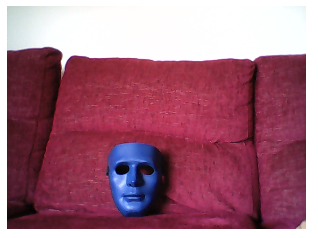
\includegraphics[width=0.65\textwidth]{figures/cf_input.png}
    \caption{Input: Fotograma de la Fuente de Vídeo}
    \label{input}
\end{figure}

Se aplicaría, en primer lugar, un suavizado a la imagen de entrada con un filtro Gaussiano para eliminar o reducir el posible ruido y, con él, los falsos positivos en el filtro. Luego convertiríamos el espacio de color de la imagen de entrada, típicamente RGB o BGR, al espacio HSV, donde resulta mucho más sencillo establecer límites para el filtrado de determinado color dado que esta característica se encuentra completamente representada en la componente H, además de ser un espacio mucho más robusto a los cambios en intensidad de luz. Por último, se aplican los límites para obtener una imagen umbral binaria en la que los píxeles de la imagen de entrada cuyo valor de la componente H está entre las cotas establecidas quedan reflejados en la imagen B/N como píxeles de primer plano (de valor 255), y el resto de píxeles se etiquetan como píxeles de fondo (de valor 0). Para señalar el objeto que supera el filtro, bastaría con hacer una aproximación rectangular a los contornos del objeto blanco de la imagen umbral (detectados en aquellas regiones en las que la derivada es muy grande, cambios rápidos de píxeles blancos a negros). Se escoge el contorno más grande localizado para asegurar la identificación de todo el conjunto de píxeles que forman el objeto. Se pueden aplicar otras técnicas para mejorar el filtrado y eliminar ruido, como operaciones morfológicas o técnicas de post-procesado.
\begin{figure}
\centering
\begin{subfigure}{.32\textwidth}
  \centering
  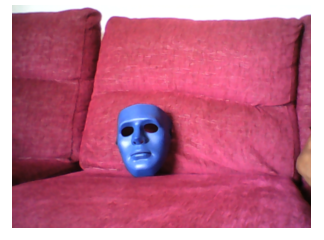
\includegraphics[width=.95\linewidth]{figures/cf_smooth.png}
  \caption{Suavizado de la Imagen}
  \label{smooth}
\end{subfigure}
\begin{subfigure}{.32\textwidth}
  \centering
  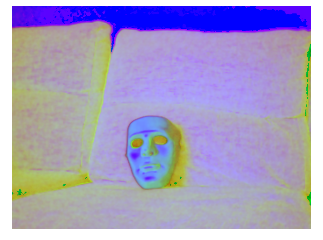
\includegraphics[width=.95\linewidth]{figures/cf_hsv.png}
  \caption{Conversión a HSV}
  \label{hsv}
\end{subfigure}
\begin{subfigure}{.32\textwidth}
  \centering
  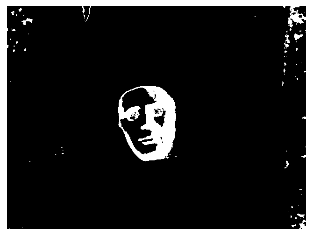
\includegraphics[width=.95\linewidth]{figures/cf_mask.png}
  \caption{Imagen Umbralizada}
  \label{mask}
\end{subfigure}
\caption{Procesado de Imagen para el Filtro de Color}
\label{procesado}
\end{figure}

El proceso descrito se muestra gráficamente en la Fig. \ref{procesado}. De esta manera, nuestro cuadernillo de Jupyter tendría ya la lógica que resuelve el filtro, además de un recubrimiento de código auxiliar que contendría el \textit{back-end} del ejercicio con los métodos de acceso a la fuente de vídeo, de recogida de imágenes, de visualización y control, etc. En la interfaz de Jupyter se pueden mostrar en todo momento las imágenes que reflejan el estado del proceso a través del API de programación de ejercicio y varias librerías gráficas (entre ellas OpenCV y matplotlib), como se ve en la Fig. \ref{ui_cf_jupyter}.

\begin{figure}[!hbtp]  \centering\noindent
    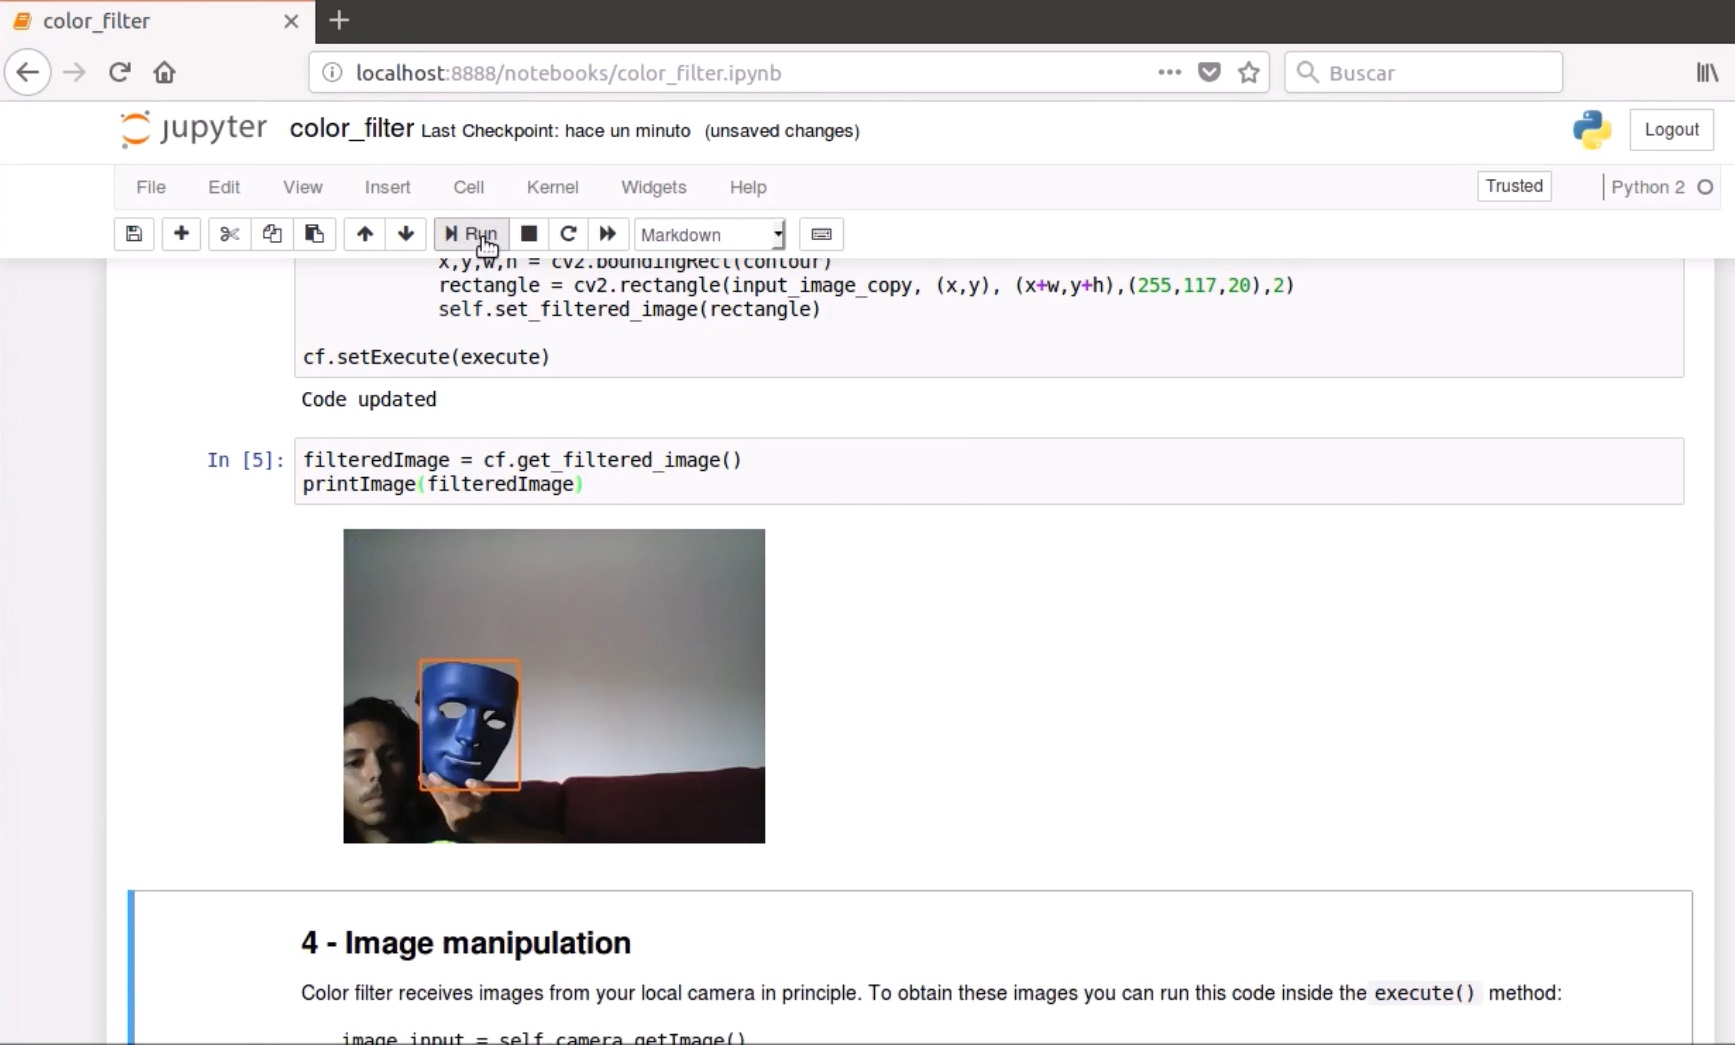
\includegraphics[width=0.99\textwidth]{figures/ui_cf_jupyter.jpg}
    \caption{UI de Jupyter para el Filtro de Color}
    \label{ui_cf_jupyter}
\end{figure}

En este punto, disponemos de una versión completamente local del prototipo de herramienta que queremos construir. Por tanto, y tras la investigación correspondiente, se procedió a la implementación de un \textit{local runtime}, es decir, de un entorno de ejecución utilizando un \textit{kernel} local. Había que desarrollar un servidor remoto que contuviese la aplicación y el modelo de ejercicio creado y que, ante una nueva petición del ejercicio, estableciese una comunicación fluida con el \textit{kernel} del cliente para coordinar la ejecución en su \textit{hardware}, por medio del lanzamiento del servidor de ``Ejecución Mixta'' en su máquina. 

Se construyó un pequeño servidor muy básico a través de Django (Fig. \ref{appui}) con capacidad para atender a un cliente que solicitase un ejercicio por medio de un click en el interfaz web, y se colocó en una máquina externa. Debajo del botón sobre el que se hace click, sucedería todo el mecanismo de enlazado y comunicación para disponer el entorno mixto.

\begin{figure}[!hbtp]  \centering\noindent
    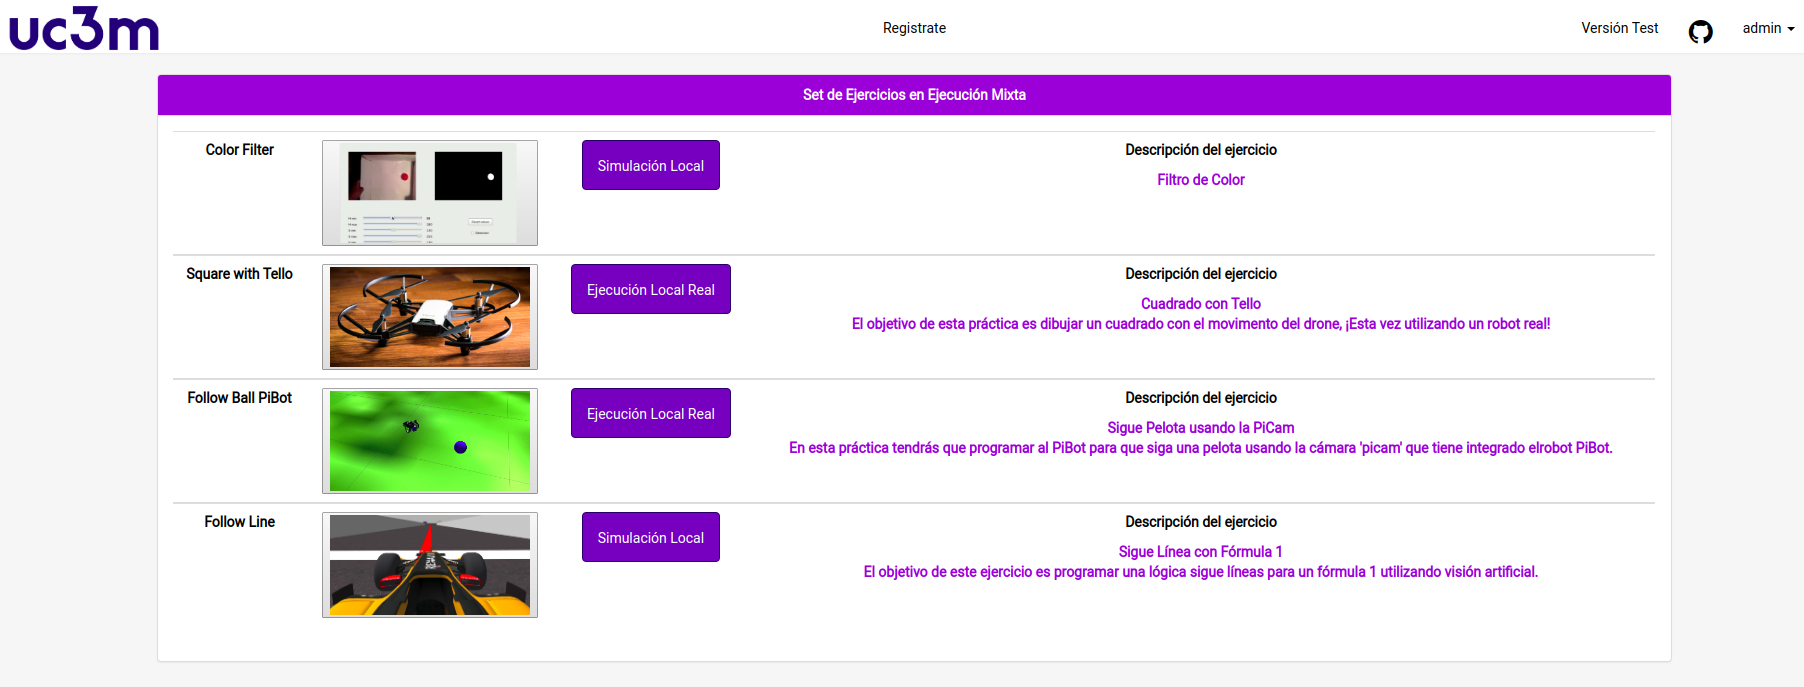
\includegraphics[width=0.99\textwidth]{figures/app_ui.png}
    \caption{UI de la Aplicación en Django}
    \label{appui}
\end{figure}

\begin{figure}[!hbtp]  \centering\noindent
    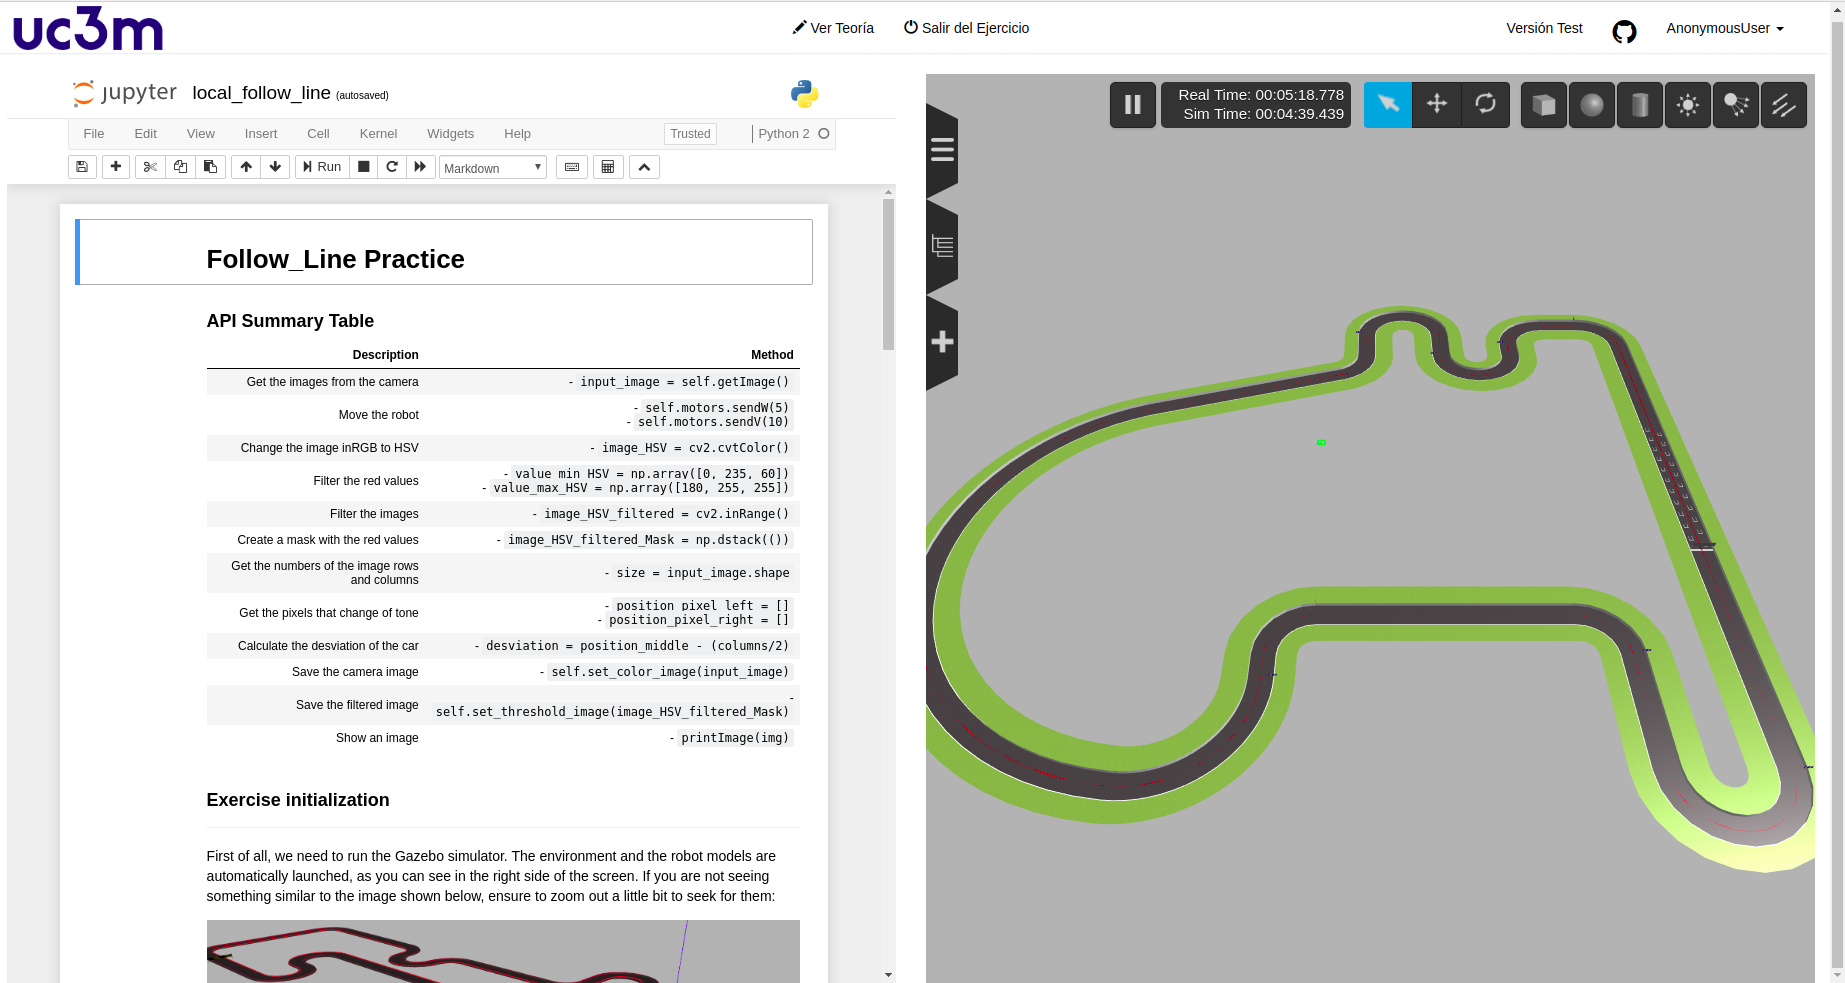
\includegraphics[width=0.99\textwidth]{figures/ui_simulation.png}
    \caption{UI de Simulación de la Aplicación}
    \label{simui}
\end{figure}

Como se puede ver en la imágenes (Fig. \ref{simui}) de la interfaz que ofrece el servidor web a su cliente, es necesario para el correcto funcionamiento de la herramienta que el receptor principal de los mensajes de ``Ejecución Mixta'' sea Jupyter, y por tanto también tiene sentido que se use como editor de código. Tras la conexión HTTPS con el servidor web, el cliente especifica su dirección IP y el puerto en que está corriendo el servidor de Jupyter en su máquina, de tal manera que se puede establecer fácilmente un puente que permita que el servidor acceda a los datos generados por Jupyter en un punto remoto, y los ofrezca al usuario como parte del interfaz, a través del mecanismo de paso de mensajes de actualización periódicos. Esto requiere hacer unos cambios sobre el servidor provisto por el proyecto Jupyter con el fin de abrir el acceso a él desde el exterior, no sin antes establecer los correspondientes métodos de seguridad. Se profundizó en la arquitectura de servicio de Jupyter para poder adaptar su funcionamiento a nuestras necesidades. Luego, como paso previo a la visualización y ejecución del código del cliente localmente a través de órdenes generadas en el interfaz ofrecido por un servidor remoto, se hace indispensable proveer al servidor de ``Ejecución Mixta'', concretamente al \textit{kernel} de Jupyter, del código asociado al ejercicio para que pueda ejecutarlo. Aquí comienza el mecanismo de establecimiento y supervisión de la conexión HTTPS de la Capa de Comunicación. La conexión con Jupyter puede hacerse de manera sencilla mediante el envío de un simple mensaje bajo el método OPTIONS, al que el servidor responderá con toda la información que necesitamos para el establecimiento de la conexión a través de cabeceras HTTP, entre ellas el \textit{token} de autenticación de Jupyter, los métodos y tipos de contenido que se aceptan, y el código CSRF\footnote{\href{https://www.geeksforgeeks.org/what-is-cross-site-request-forgery-csrf/}{What is CSRF and how to prevent it?}} necesario para enviar información al servidor.

Estudiamos el mecanismo de comunicación de la plataforma, que emplea principalmente el protocolo ZeroMQ\footnote{\url{https://zeromq.org/}} o 0MQ para el intercambio asíncrono de mensajes \textit{N-a-N} a través de la web. Esto nos proporciona, además de una plantilla para los tipos de mensajes que debemos enviar al \textit{kernel} de Jupyter, una idea bastante fiel del proceso que desencadena cada órden o petición que se le hace al servidor de Jupyter. También se utilizó \textit{sniffers}\footnote{\href{https://www.wireshark.org/\#1398253364-1-69}{Wireshark Sniffer}} para monitorizar el funcionamiento local de Jupyter (Fig. \ref{wireshark}). Este paso fue vital para comprender el procedimiento que debíamos seguir para iniciar una sesión de Jupyter completa y válida.

\begin{figure}[!hbtp]  \centering\noindent
    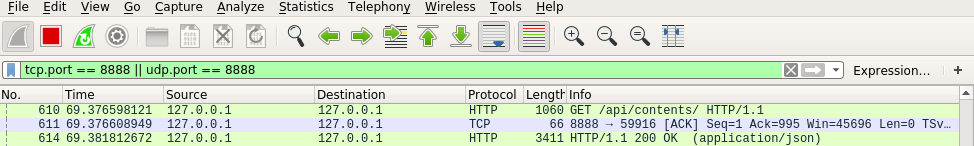
\includegraphics[width=0.99\textwidth]{figures/wireshark.png}
    \caption{Capura de Paquetes del Mecanismo de Comunicación de Jupyter}
    \label{wireshark}
\end{figure}

Tras el establecimiento, se puede comenzar con el intercambio de mensajes 0MQ. Aprovecharemos el REST API que ofrece Jupyter para la comunicación con el \textit{kernel} en tanto que este \textit{RESTfull Service}\footnote{\href{https://docs.oracle.com/javaee/6/tutorial/doc/gijqy.html}{What is a RESTfull Service?}} ofrece todo lo necesario para enviarle ficheros de código, órdenes de ejecución, órdenes de control (reinicio, apagado, encendido, pausa, cambio de lenguaje, limpieza de salidas, etc.) (Fig. \ref{jupyter_rest_api}) y, en general, lo necesario para facilitar el uso de la plataforma a través de la web. Por tanto, por el canal de ``Ejecución Mixta'' estaríamos enviando, principalmente, mensajes HTTP sobre una capa de TLS con datos de tipo 0MQ en el cuerpo, destinados a Jupyter.

\begin{figure}[!hbtp]  \centering\noindent
    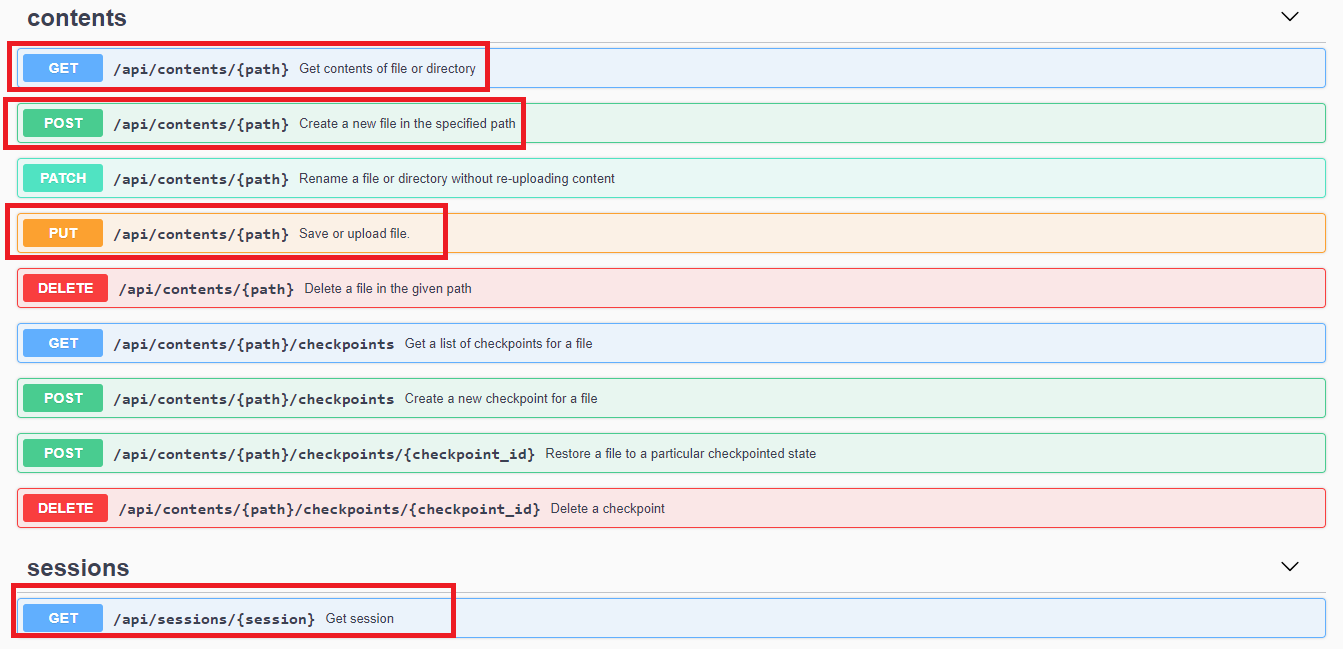
\includegraphics[width=0.99\textwidth]{figures/jupyter_rest_api.png}
    \caption{REST API de Jupyter}
    \label{jupyter_rest_api}
\end{figure}

En base al conocimiento obtenido del motor de comunicación de Jupyter, seleccionamos aquellos métodos del REST API que necesitaríamos, marcados en la imagen superior. Se muestra a continuación un ejemplo del mensaje que se enviaría al servidor de Jupyter para hacer llegar el código al \textit{kernel} encargado de un cuadernillo concreto:

\lstset{
   language=JavaScript,
   backgroundcolor=\color{lightgray},
   extendedchars=true,
   basicstyle=\footnotesize\ttfamily,
   showstringspaces=false,
   showspaces=false,
   numbers=left,
   numberstyle=\footnotesize,
   numbersep=9pt,
   tabsize=2,
   breaklines=true,
   showtabs=false,
   captionpos=b
}
\begin{minipage}{\linewidth}
\begin{lstlisting}[caption=Formato de Mensajes de ``Ejecución Mixta'']
const url = 'http://'+_ip+':'+_port+'/api/contents/' + nbname;
const data_put = ' {"type": "notebook",
                    "format": "json",
                    "content": ' + nbcontent + '} ';
const message = {
        headers:{'Content-Type':'application/json',
                 //'Authorization': 'token ' + _token,
                },
        body:data_put,
        method:"PUT"
};
\end{lstlisting}
\end{minipage}

donde cada variable que aparece en el mensaje (\textit{\_ip, \_port, nbname,\_token, nbcontent}) sería establecida por el servidor web y contendría la dirección del servidor Jupyter y el contenido y nombre del cuadernillo que queremos enviar. El formato de todos los mensajes es similar, en tanto que se trata de peticiones HTTP como se puede ver en la constante \textit{message} con el formato de cuerpo 0MQ que se refleja en la constante \textit{data\_put}. Este tipo de mensajes, con su respectiva codificación, constituye el tipo de mensajes a intercambiar por la herramienta ``Ejecución Mixta'' para el establecimiento y envío iniciales.

El proceso de comunicación con Jupyter comenzaría por el establecimiento de la conexión, donde se crea una sesión de ejecución, continuaría con el envío del código del cuadernillo y de cada fichero de código de aplicación auxiliar que necesite el ejercicio, para acabar con una orden de inicio del \textit{kernel} del lenguaje adecuado encargado de la ejecución, que se montará sobre un núcleo latente en el sistema del cliente web. La utilización de direcciones IP públicas, el protocolo HTTP (estándar de Internet) que utiliza por defecto el puerto 8080 (puerto de Internet, abierto a mensajes transportados sobre TCP o UDP por la red, con cualquier origen) que puede atravesar \textit{firewalls} y resolver conexiones sea cual sea el dominio público, y el \textit{token} de autorización embebido en los mensajes garantizan la conectividad y la integridad de la sesión de Jupyter, así cómo el funcionamiento entre sistemas bajo distintas redes o sub-redes de la misma red.

En este punto del desarrollo, hemos superado el principal obstáculo de la ``Ejecución Mixta'' e implementado un mecanismo capaz de ejecutar código entre redes, con actualización de los resultados en tiempo real en ambos lados servidor  y cliente web. Se completa así el primer ciclo de trabajo, no sin antes realizar los tests convenientes de funcionamiento y desempeño y el análisis de los resultados. La herramienta ya es capaz de conectar un código remoto (aplicación robótica) con un ``robot'' local (cámara). Se propusieron los siguientes pasos y analizaron los riesgos, donde salió a la luz la necesidad de utilizar contenedores Docker (lo cual cambiará sustancialmente el mecanismo de comunicación) y la posibilidad de enriquecer la aplicación robótica con otros procesos dentro de él, para dar soporte de simulación y ampliar el \textit{hardware} utilizable.

Hubo que estudiar el motor de Docker y su funcionamiento para crear un \textit{DockerFile} con instrucciones en lenguaje SHELL para virtualizar una distribución Ubuntu con todas las herramientas y aplicaciones auxiliares involucradas en la ``Ejecución Mixta'', para que utilizar la herramienta resultase tan fácil como descargar la imagen Docker y levantar el contenedor. Utilizar un contenedor Docker para empaquetar los procesos necesarios e incluir seguridad supone añadir complejidad el mecanismo de comunicación, en tanto que Docker levanta su propia sub-red dentro de la red del cliente, lo que nos deja una intratable sub-red dentro de una red distinta desde el punto de vista del servidor web. Se replanteó el mecanismo de comunicación para que utilizase el navegador del cliente web como intermediario entre el usuario y la aplicación robótica, el cual sí que tiene conectividad directa con una sub-red de su propia red. Por tanto, el servidor web abre ahora una comunicación con el \textit{browser} del cliente en lugar de directamente con el servidor Jupyter, y éste actúa como \textit{proxy} reenviando cada mensaje donde corresponde a través de una secuenciación programada en código JavaScript, de manera que tanto de cara al cliente como al servidor web, la comunicación sigue siendo la misma que en el paso anterior, esta vez con un origen o destinatario distinto. Simplemente se trata de añadir la lógica del \textit{proxy} para que viaje con la aplicación que se sirve al usuario web. El navegador ya utiliza protocolos como STUN o ICE que permiten descubrir e interaccionar con ambas partes del mecanismo. Así, los mensajes reenviados por el navegador serán recibidos por el módulo secuenciador de ``Ejecución Mixta'', que procesará la información que llega para orquestar el correcto inicio del entorno y los agentes, traduciendo las órdenes JavaScript iniciales a comandos de lanzamiento (Listing. 5.2) y entregando las órdenes de ejecución a quien corresponda (Listing. 5.3). Ahora se tiene un prototipo completo y seguro, capaz de funcionar sobre Docker y a través de Internet, con ambos extremos situados en cualquier punto.

\begin{lstlisting}[language=bash, caption=Código de Inicio del Secuenciador]
#!/bin/bash

rm -rf /tmp/.X0-lock

Xvfb -shmem -screen 0 1280x1024x24 &

source /opt/jderobot/setup.bash
source /opt/ros/kinetic/setup.bash
source /opt/jderobot/share/jderobot/gazebo/gazebo-assets-setup.sh
export PYTHONPATH=$PYTHONPATH:/home/jderobot/.exercises

cd ~/gzweb
npm start &

cd ~/volume/user/exercise

jupyter nbextension enable hide_input/main --user
jupyter nbextension enable init_cell/main --user
jupyter notebook --ip=0.0.0.0 --allow-root &

cd ~

EXTENSION=`echo "$1" | cut -d'.' -f2`
if [ $EXTENSION = "world" ]
  then
    roscore &
fi

if ! [ -z "$2" ]
  then
    python ~/referees/$2 &
fi

if ! [ -z "$1" ]
  then
    EXTENSION=`echo "$1" | cut -d'.' -f2`
    if [ $EXTENSION = "launch" ]
      then
        roslaunch /opt/jderobot/share/jderobot/gazebo/launch/$1
    else
        rosrun gazebo_ros gazebo /opt/jderobot/share/jderobot/gazebo/worlds/$1
    fi
else
    tail -f /dev/null
fi
\end{lstlisting}
\begin{lstlisting}[language=bash, caption=Reenvío de Mensajes]
[I 11:51:09.187 NotebookApp] Saving file at /thumbnail_follow_line.png
[Gazebo] Sat Jan 11 2020 11:51:09 GMT+0000 (Coordinated Universal Time) Received Message: {"op":"advertise","id":"advertise:~/heartbeat:14","type":"heartbeat","topic":"~/heartbeat"} from http://127.0.0.1:8080 ::ffff:172.17.0.1
[Python Process] Sat Jan 11 2020 11:51:09 GMT+0000 (Coordinated Universal Time) Received Message: {"op":"publish","id":"publish:~/heartbeat:15","topic":"~/heartbeat","msg":{"alive":1}} from http://127.0.0.1:8080 ::ffff:172.17.0.1
[I 11:51:11.758 NotebookApp] 302 GET /notebooks/world.png (172.17.0.1) 0.95ms
[I 11:51:11.847 NotebookApp] Adapting to protocol v5.1 for kernel 368a1e46-acc2-4976-acf3-25528ae77d77
\end{lstlisting}

El API de inicio de la ``Ejecución Mixta'' fue enriquecido con la aparición de los parámetros característicos de Docker que permiten crear un puente seguro entre un elemento virtualizado y su homólogo en la máquina anfitrión. Un ejemplo de esto es el mecanismo que ya anticipábamos para el acceso a la cámara integrada en el sistema cliente desde el interior de un contenedor Docker, resuelto con el mapeo \textit{-v /dev/video0:/dev/video0}, o la redirección de interfaces de escucha del sistema a sus correspondientes dentro del contenedor (\textit{-p 8888:8888 -p 8889:8889 -p 8080:8080}).

Llegados a este punto, se trata de enriquecer la ``Ejecución Mixta'' para que además de ejecutar lógica pueda simular y usar aplicaciones auxiliares como \textit{plugins} o \textit{drivers} robóticos. Utilizamos ROS dada su fácil integración con Gazebo y el lenguaje Python, que nos permite construir una aplicación completa y autocontenida asociada al código del ejercicio que, lanzada en el interior del contenedor de ``Ejecución Mixta'', creará el mecanismo de inter-comunicación a través de mensajes de ROS que orquestará el funcionamiento de un código que se ejecuta en una aplicación para que sus resultados se reflejen en la simulación y en la aplicación web al mismo tiempo. Lo mismo sucederá con robots reales sustituyendo el simulador por un controlador del dispositivo \textit{hardware}, empleando el mismo mecanismo interno de mensajes (Listings. 5.4 y 5.5). Cada mensaje que deba viajar hacia la aplicación con información relevante será recogido a través de un canal WebSockets por el secuenciador del módulo de gestión situado en el navegador, envuelto con una capa HTTPS y enviado al servidor remoto para que este lo procese (Fig. \ref{mixedexecarch}).

\begin{lstlisting}[language=bash, caption=Topics de ROS asociados a los Canales de Comunicación Internos]
~$ rostopic list
/F1ROS/cameraL/camera_info
/F1ROS/cameraL/image_raw
/F1ROS/cameraL/parameter_descriptions
/F1ROS/cameraL/parameter_updates
/F1ROS/cmd_vel
/F1ROS/odom
/clock
/gazebo/link_states
/gazebo/model_states
/gazebo/parameter_descriptions
/gazebo/parameter_updates
/gazebo/set_link_state
/gazebo/set_model_state
/rosout
/rosout_agg
/tf
\end{lstlisting}

\begin{minted}[
    gobble=4,
    frame=single,
    linenos
  ]{yaml}
    # follow_line.yml
    Camera:
      Topic: "/F1ROS/cameraL/image_raw" 
      Name: follow_line_camera
    
    
    Motors:
      Topic: "/F1ROS/cmd_vel"
      Name: follow_line_motors
      MaxV: 40
      MaxW: 2
    
    Websockets:
      Host: 0.0.0.0 
      Port: 9002
      SSL: False
      Cert: '/etc/certs/fullchain1.pem' 
      Key: '/etc/certs/privkey1.pem'
\end{minted}
\begin{lstlisting}[caption=Configuración de Canales del Secuenciador en formato YAML]
\end{lstlisting}

Una vez dispuesto el contenedor Docker, completamos otro ciclo y verificamos que la ``Ejecución Mixta'' ya no supone ninguna carga de cómputo para el lado servidor de la aplicación web, y también que podemos eliminar el proceso de instalación, dado que todas las dependencias están agrupadas en el contenedor. Lanzar la ``Ejecución Mixta'' pasa ahora por utilizar el API de Docker de control de contenedores, que pondrá en marcha todos los sub-sistemas necesarios para el funcionamiento de la aplicación robótica y los dejará disponibles para su consulta desde el exterior, por parte del servidor remoto a través del secuenciador o \textit{proxy} web. Así, la aplicación puede enviar cualquier tipo de orden de ejecución en formato Python al servidor de Jupyter, que materializará esa orden en el simulador Gazebo a través de los canales ROS o, incluso, en el robot o sensor real conectado al sistema del cliente. La aplicación robótica le indicará al secuenciador qué sub-procesos necesita para el funcionamiento de un ejercicio robótico concreto.

Para implementar el soporte de simulación, se diseñó un sistema de configuración que permite indicar los elementos, robots y características que debe tener la escena simulada a través de Gazebo (Fig. \ref{gzworld}), haciendo uso de ficheros de extensión \textit{.world} o \textit{.launch}, siendo los primeros un subconjunto del lenguaje de marcado XML que indica los agentes involucrados en la simulación (Listing. 5.7), y el segundo un configurador inteligente que permite lanzar, además del mundo de simulación, una serie de nodos que se puedan necesitar para controlar por ejemplo las interfaces de un determinado robot (Listing. 5.6). 

\begin{lstlisting}[language=XML, caption=Configuración de Lanzamiento de Simulaciones]
<?xml version="1.0" encoding="UTF-8"?>
<launch>
  <!-- We resume the logic in empty_world.launch, changing only the name of the world to be launched -->
  <include file="$(find gazebo_ros)/launch/empty_world.launch">
    <arg name="world_name" value="f1_1_simplecircuit.world"/> <!-- Note: the world_name is with respect to GAZEBO_RESOURCE_PATH environmental variable -->
    <arg name="paused" value="false"/>
    <arg name="use_sim_time" value="true"/>
    <arg name="gui" value="true"/>
    <arg name="headless" value="false"/>
    <arg name="debug" value="false"/>
    <arg name="verbose" default="false"/>
  </include>  
</launch>
\end{lstlisting}

\begin{lstlisting}[language=XML, caption=Configuración de Lanzamiento de Simulaciones]
<?xml version="1.0" ?>
<sdf version="1.5">
  <world name="default">
    <scene>
      <grid>false</grid>
    </scene>
    <!-- A global light source -->
    <include>
      <uri>model://sun</uri>
    </include>
    <include>
	    <uri>model://pista_simple</uri>
	    <pose>0 0 0 0 0 0</pose>
    </include>
    <include>
      <uri>model://f1_renault</uri>
      <pose>53.462 -10.734 0.004 0 0 -1.57</pose>
    </include>
    <scene>
        <sky>
            <clouds>
                <speed>12</speed>
            </clouds>
        </sky>
     </scene>
  </world>
</sdf>
\end{lstlisting}

\begin{figure}[!hbtp]  \centering\noindent
    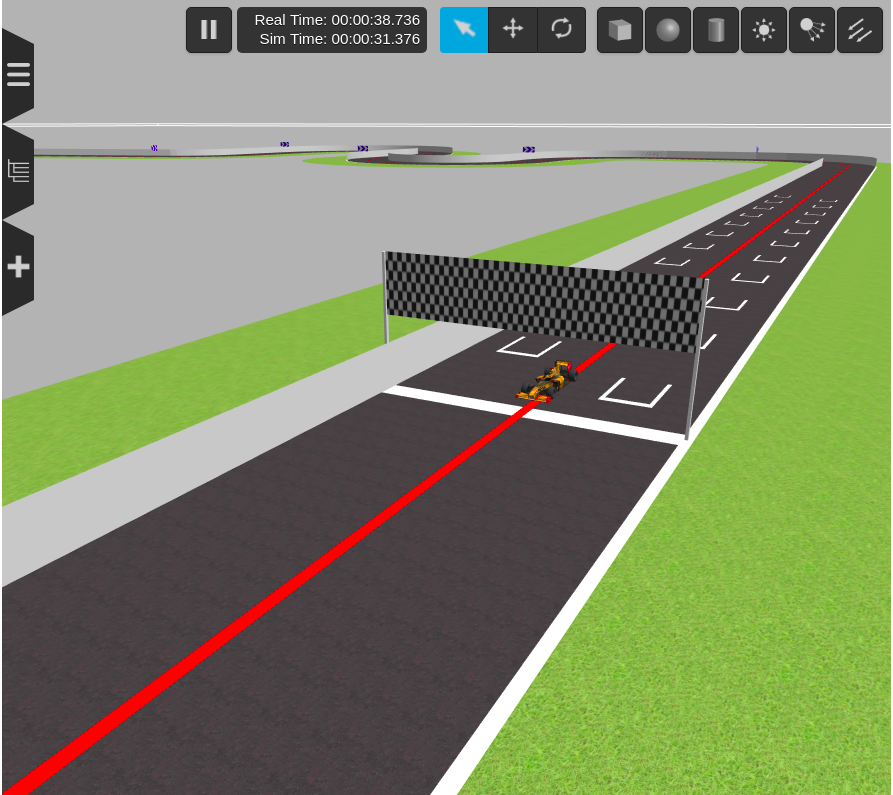
\includegraphics[width=0.9\textwidth]{figures/world_gazebo.png}
    \caption{Escenario de Simulación}
    \label{gzworld}
\end{figure}

Con ello, al lanzar la herramienta se indicará qué fichero de configuración se quiere usar a través de instrucciones del API de ``Ejecución Mixta'', que se ocupará de levantar tanto la simulación como la red de comunicación interna basada en ROS como se puede ver en el \textit{snippet} de código inferior (Listing. 5.8), y la capa de abstracción que permite al usuario programar su robot y acceder a toda la funcionalidad mientras se materializan los cambios en el simulador.

\begin{minted}[
    gobble=4,
    frame=single,
    linenos
  ]{python}
    class ListenerCamera:
        def __init__(self, topic):
            
            self.topic = topic
            self.data = Image()
    
        # [...]
    
        def start (self):
     
            self.sub = rospy.Subscriber(self.topic, ImageROS,
                                        self.__callback)
    
    class PublisherMotors:
     
        def __init__(self, topic, maxV, maxW):
    
            self.maxW = maxW
            self.maxV = maxV
    
            self.topic = topic
            self.data = CMDVel()
            self.pub = rospy.Publisher(self.topic,
                                       Twist,
                                       queue_size=1)
            rospy.init_node("FollowLineF1")
    
        # [...]
    
        def publish (self):
    
            self.lock.acquire()
            tw = cmdvel2Twist(self.data)
            self.lock.release()
            self.pub.publish(tw)
    
    class FollowLine():
        
        def __init__(self):
            cfg = readConfig()
    
            cameraTopic = cfg["Camera"]["Topic"]
            motorsTopic = cfg["Motors"]["Topic"]
            maxv = cfg["Motors"]["MaxV"]
            maxw = cfg["Motors"]["MaxW"]
    
            self.camera = ListenerCamera(cameraTopic)
            self.motors = PublisherMotors(motorsTopic, maxv,
                                          maxw)
    
            # [...]
\end{minted}
\begin{lstlisting}[caption=Creación de la Red Interna de Comunicación]
\end{lstlisting}

Con todo lo anterior ya resuelto, decidimos implementar también el soporte de ejecución compartida haciendo uso de robots reales. Dada la filosofía modular interconectada que se había diseñado hasta este momento, el enfoque para el caso de querer controlar un robot real desde el lado cliente pasaba sencillamente por crear su controlador, e incluirlo como aplicación auxiliar lanzada dentro de la herramienta y orquestada como un módulo más por el secuenciador. Así, se implementó un driver casero para el robot Tello (Listing. 5.9), un cuadricóptero de DJI e Intel cuyo precio de mercado está al alcance del consumidor medio. Una vez hecho el driver en lenguaje Python, se creó un paquete PIP con el objetivo de poder utilizarlo desde el código del usuario, el cual lo importa como una librería normal y corriente y accede a sus funciones y métodos públicos para controlar el dron (Listing. 5.10). 

\begin{minted}[
    gobble=4,
    frame=single,
    linenos
  ]{python}
    #!/usr/bin/env python
    # -*- coding: utf-8 -*-
    
    import socket, threading, time, libh264decoder, cv2
    import numpy as np
    from math import pi as PI
    from speed_thread import SpeedThread
    
    MAX_VEL = 1.5 # m/s
    MIN_VEL = 0.1 # m/s
    MAX_ROT_VEL = 1 # deg/s
    MAX_ROT_VEL = 360 # deg/s
    ORANGE_MIN = np.array([117, 239, 76],np.uint8)
    ORANGE_MAX = np.array([179, 255, 255],np.uint8)
    
    class Tello:
        """Wrapper class to interact with the Tello drone."""
        def __init__(self, local_ip, local_port,
        command_timeout=.2, tello_ip='192.168.10.1',
                     tello_port=8889):
            # vels vector
            #   [
            #       Right(+)/Left(-),
            #       Forward(+)/Backward(-),
            #       Up(+)/Down(-),
            #       Yaw_right(+)/Yaw_left(-)
            #   ]
            self._vels = [0, 0, 0, 0]
            self.abort_flag = False
            self.decoder = libh264decoder.H264Decoder()
            self.command_timeout = command_timeout
            self.response = None  
            self.frame = None  # numpy array BGR
    
            # socket for sending cmd
            # -------------------------------------------
            self.socket = socket.socket(socket.AF_INET,
                                        socket.SOCK_DGRAM)  
            self.tello_address = (tello_ip, tello_port)
            self.socket.bind((local_ip, local_port))
            # -------------------------------------------
    
            # thread for speed control
            # -------------------------------------------
            self.kill_event = threading.Event()
            self.speed_thread = SpeedThread(self)
            # -------------------------------------------
    
            print("Conectando con Tello .....")
            # to receive video -- send cmd: command, streamon
            self.socket.sendto(b'command', self.tello_address)
            print ('[Tello] Preparando controlador')
            self.socket.sendto(b'streamon', self.tello_address)
            print ('[Tello] Preparando flujo de vídeo')
    
            # [...]
\end{minted}
\begin{lstlisting}[caption=Snippet del Driver de Tello]
\end{lstlisting}

\begin{minted}[
    gobble=4,
    frame=single,
    linenos
  ]{python}
    from tello.tello_wrapper import Drone
    tel = Drone('', 9005)
\end{minted}
\begin{lstlisting}[caption=Uso del Driver]
\end{lstlisting}


De manera análoga a lo ya construido, se diseñaron algunos ejercicios más para probar la herramienta bajo distintos pretextos.

\section{Funcionamiento}
\subsection{Flujograma}

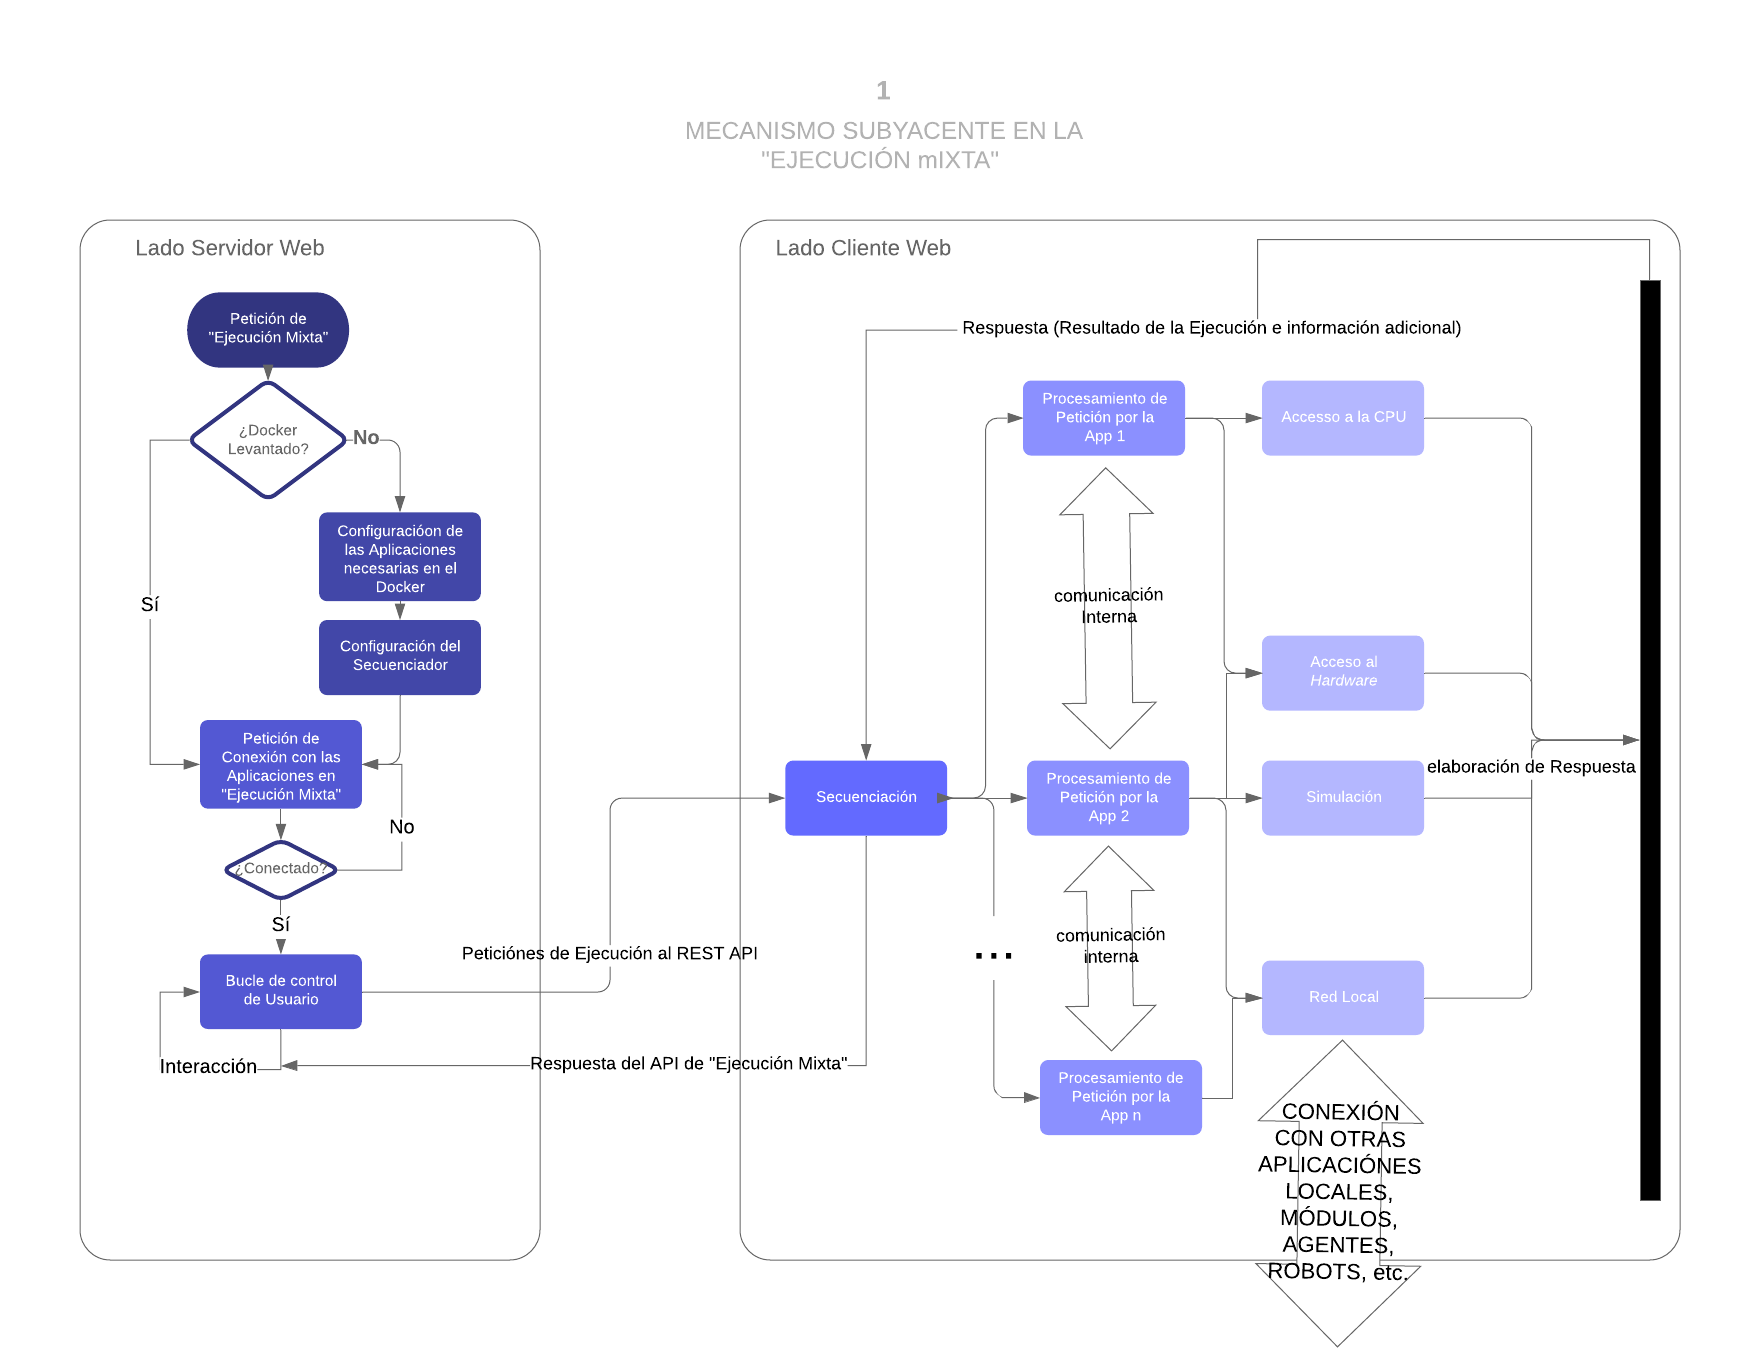
\includepdf[addtolist={1,figure,{Flujograma},flowchart}]{figures/flowchart.png}

\subsection{Mecanismo subyacente de la Herramienta}

Para explicar el mecanismo que desata el uso de la ``Ejecución Mixta'' por parte de una aplicación, se utilizará el caso hipotético de un usuario que dispone de un robot móvil con conectividad inalámbrica a través de una red propia con visibilidad a la red local del usuario, al ser la del robot una subred de ésta.

Apoyándonos en el diagrama de flujo anterior (Fig. \ref{flowchart}), el proceso comienza con la realización de la petición inicial de ``Ejecución Mixta'', que se corresponde con la solicitud hecha por el usuario a la aplicación remota de un servicio que utiliza senda herramienta de ejecución. Dado que la aplicación web remota es la que ofrece el servicio solicitado, es también la aplicación la que conoce la configuración de ``Ejecución Mixta'' necesaria para el proceso, así como la combinación de aplicaciones de las que va a requerir información durante la ejecución que deben iniciarse en el lado cliente web. Es entonces cuando se envía esta configuración al cliente, quien debe iniciar el contenedor Docker que aloja la herramienta. Una vez iniciado, se ha de conectar con cada una de las aplicaciones contenidas en la herramienta de ejecución desde la aplicación web. Como se mencionó con anterioridad, esto desencadena en el servidor web una petición inicial al API de ``Ejecución Mixta'', que pasa a desempeñar el rol de cliente de ``Ejecución Mixta'', y que hace una solicitud de conexión. Si los mecanismos de seguridad se resuelven con éxito, el secuenciador del lado cliente web, que actúa como servidor de ``Ejecución Mixta'', garantiza el acceso de la aplicación remota a la ejecución. Es entonces cuando se inicia el servicio que el cliente web solicitó en primera instancia, ingresando en un bucle de control y eventos de la misma forma que sucedería en cualquier otro tipo de aplicación web. En este bucle, la aplicación web atiende permanentemente las interacciones del usuario web, quien generará eventos en el contexto de la aplicación web, y que podrá generar peticiones concretas de ejecución local. Cuando se produce este tipo de petición es cuando la aplicación hace uso de la ``Ejecución Mixta'' para lanzar el código del usuario web, escrito y almacenado remotamente desde su punto de vista, sobre el \textit{hardware} local al usuario. Como se comentó, estas peticiones viajan con un formato concreto a modo de protocolo con destino al secuenciador de ``Ejecución Mixta'', quien ya en el entorno local es capaz de analizar la petición y redirigirla convenientemente a su destinatario o destinatarios. Los receptores finales de estas solicitudes serán las diferentes aplicaciones lanzadas para soportar el servicio web, que se especificaban en el \textit{entrypoint} de configuración inicial del secuenciador. Es entonces cuando los receptores pueden procesar la petición, siempre y cuando el método solicitado esté soportado por el REST API de ``Ejecución Mixta''. El receptor principal será siempre Jupyter, pues es quién tendrá la capacidad de ejecutar código sobre la CPU local o el robot. También habrá un volumen considerable de peticiones de simulación, con el fin de mantener siempre actualizado el estado de la simulación, si existe, en la aplicación web y su interfaz gráfico, que es el que ve el usuario. Para el caso planteado, incluso habrá peticiones concretas o resultados de la ejecución del código que desembocarán en el establecimiento de un nuevo canal de comunicación a través de la red del cliente web. Como se puede ver en el diagrama anterior, este canal se puede utilizar para conectar el resultado de la ``Ejecución Mixta'' a cualquier otra aplicación externa del lado servidor de ejecución preparada para recibir los mensajes de respuesta que se generan. Esto hace crecer la potencia y el alcance de la ejecución, y las posibilidades de servicio web que se puede ofrecer. En el caso del ejemplo, la ejecución generaría mensajes que deben ser enviados al receptor del robot móvil a través de la red inalámbrica, que se materializarían en la actualización de sus actuadores y sensores. Según sea el mensaje, el robot devolverá cierta información. Con esta información, y la proveniente del resultado del procesamiento de la petición entrante por cada aplicación receptora, se compone un único mensaje de respuesta que se reenvía a través del API al servidor web, con toda la información que el servicio espera para su correcto funcionamiento. El ejemplo para este caso pueden ser mensajes de éxito o fracaso de acceso a las interfaces del robot y el resultado concreto de la ejecución solicitada. La información se usa en última instancia para actualizar el interfaz y el estado del servicio para que el cliente web pueda ver el resultado de su interacción. Se finalizaría así la iteración del proceso de ``Ejecución Mixta'' y quedaría a la espera de nuevas peticiones hasta la solicitud de finalización de ejecución, con la cual se liberaría la memoria asignada a todos los procesos en el lado servidor de ejecución y se detendría el contenedor de forma segura, pudiéndose dar por terminado el servicio web.